%================================================================
\section{Results and Discussion}\label{sec:Results}
%================================================================

%----------------------------------------------------------------
\subsection{Verification of the Implementation}\label{sec:project results}
%----------------------------------------------------------------

\autoref{fig:grid_search} shows the VMC computations of the expected energy and the corresponding variance with both the analytical and automatic differentiation approaches for a system of $N=1, 10, 100, 500$ non-interacting bosons in a spherical harmonic oscillator. We here use a grid search for the optimal variational parameter which is computationally expensive and generally infeasible for a non-coarse grid. However, in this case where we know the exact values, a grid search with a grid containing the exact value can be used to validate the sampling approach and implementation. As can be seen in the figure, the exact energy $\expval{E}/N = 3/2 \, \hbar \omega_\mathrm{ho}$ with $\Var \qty(E) / N = 0$ at $\alpha=1/2$ are found by both approaches, which indicates that the sampler works well and the implementation of the system is correct. The figure also illustrates the convex nature of the variational parameter optimization problem. In this study we optimize the variational parameter with respect to the expectation value of the energy, as described in \autoref{sec:gradient_descent}. However, the figure indicates that the variance might be more optimal as the optimization target since it tends to yield rather large values for non-optimal variational parameter values. 

%shows VMC computations for a grid of $\alpha$ values for a non-interacting system with spherical potential with $500$ particles for both the analytical and automatic differentiation approaches. Both approaches find the exact energy of the ground state when $\alpha=0.5$. The regularity of the curve indicates that the sampling is performed well. However, for large $\alpha$ values, the sampler seems to run into some minor issues, as the sampled energy does not behave as regularly as desired. When $\alpha$ increases, the Gaussian wave function becomes a sharper peak, and there may be a need for more tuning or warm-up cycles before sampling.

\begin{figure}[!htb]
\centering
\subfloat[]{{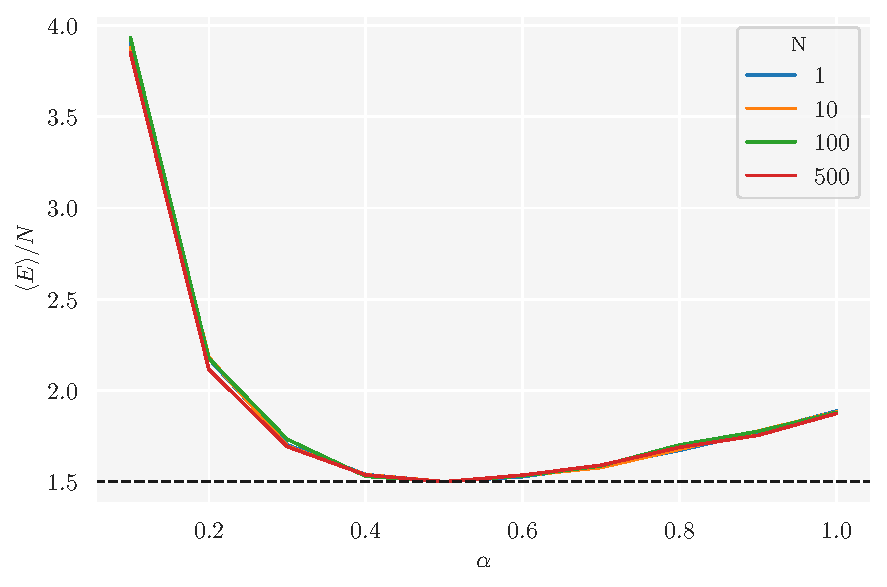
\includegraphics[scale=0.5]{latex/figures/grid_search_ashonib_rwm_energy.pdf}}}
\qquad
\subfloat[]{{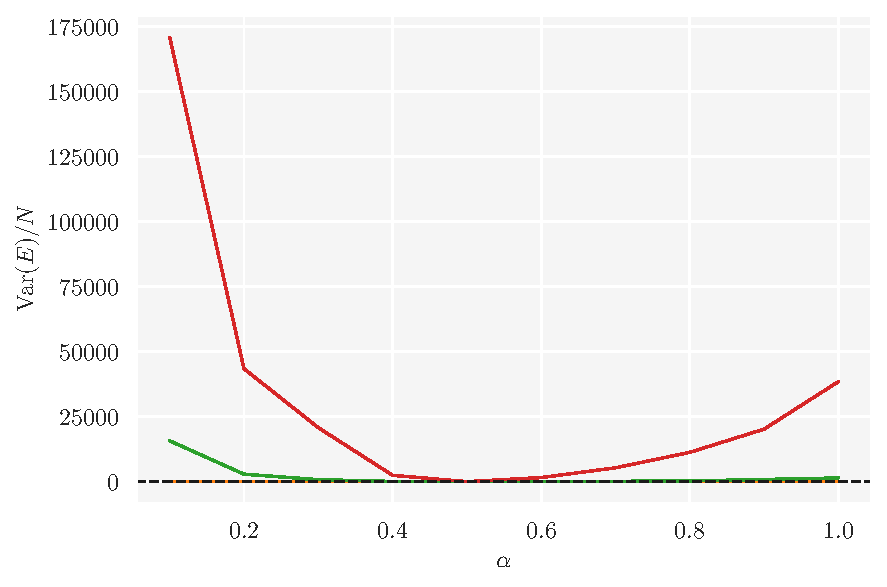
\includegraphics[scale=0.5]{latex/figures/grid_search_ashonib_rwm_variance.pdf}}}
\qquad
\subfloat[]{{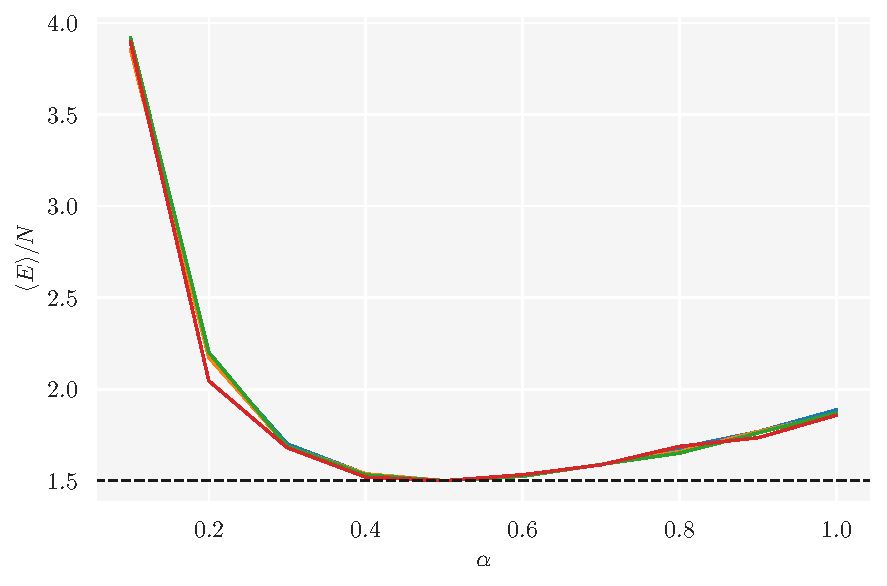
\includegraphics[scale=0.5]{latex/figures/grid_search_shonib_rwm_energy.pdf}}}
\qquad
\subfloat[]{{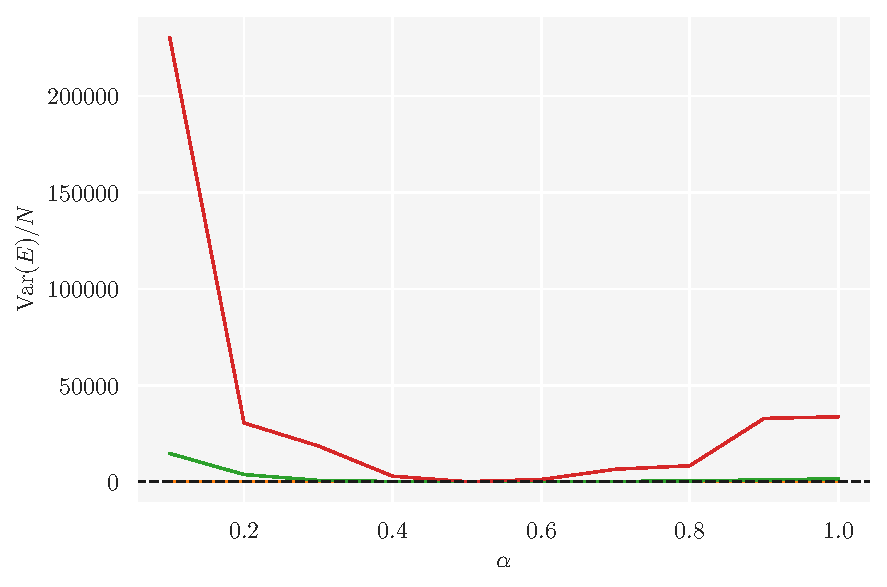
\includegraphics[scale=0.5]{latex/figures/grid_search_shonib_rwm_variance.pdf}}}
\caption{The expected value of the energy, $\expval{E}$, and variance, $\Var \qty(E)$, scaled  by the number of bosons, $N$, in a grid search for the optimal variational parameter $\alpha$. The system is a spherical harmonic oscillator with non-interacting bosons and the grid of variational parameters $\alpha \in [0.1, 1.0]$ with step size $0.1$. In \textbf{(a)} and \textbf{(b)} the expectation values are computed with the closed-form expressions, whereas in \textbf{(c)} and \textbf{(d)} the computations are done with automatic differentiation through JAX. Each computed point in the grid is the average over 16 tuned Markov chains with $20,000$ energy samples used to calculate the expectation values in each.}
\label{fig:grid_search}
\end{figure}

\autoref{tab:verification_energy} tabulates the computed expectation values of the energy using the same spatial configuration of interacting bosons in a spherical harmonic oscillator with two different implementations. One implementation is based on closed-form expressions in the linear domain whereas the other on closed-form expressions in the logarithmic domain (see \autoref{sec:analytical_interact}). As can be seen in the table, the expected energy calculations are identical for a given system size. As the implemented closed-form expressions found by different routes are identical, this further indicates the validity of the implementation.

\begin{table}[!htb]
\caption{Comparison between the implementation of analytical expressions for a system of interacting of bosons in a spherical harmonic oscillator. One is performed in the linear domain and the other in the log domain.}
\centering
\rowcolors{2}{gray!25}{white}
\begin{tabular}{ccc}
\hline
\hline 
\# of bosons & $\expval{E}$ linear domain & $\expval{E}$ log domain
\\
\hline 
\hline 
                   2 &         3.001 &                    3.001 \\
                   5 &         7.512 &                    7.512 \\
                  10 &        15.052 &                   15.052 \\
                  20 &        30.236 &                   30.236 \\
                  50 &        76.497 &                   76.497 \\
                 100 &       155.915 &                  155.915 \\
                 200 &       324.771 &                  324.771 \\
                 500 &       897.372 &                  897.372 \\
                1000 &     2,095.517 &                2,095.517 \\
\hline
\end{tabular}
\label{tab:verification_energy}
\end{table}

\autoref{fig:trace_phase} shows the three phases of the sampler for both the RWM and LMH algorithms used on a system of $N=100$ bosons in a spherical trap both with and without interactions. First, the sampler tunes the proposal scale parameter by increasing or decreasing it according to a look-up table (see \cw{vmc/utils/sampler_utils.py} in the source code) that tries to achieve a target acceptance rate. Then, the sampler search for the optimal variational parameter by employing gradient descent optimization, specifically, the ADAM optimizer discussed in \autoref{sec:adam}. The updates in the tuning and optimization phases are done after a set interval of MCMC steps. Both the tuning and optimization phase also employs early stopping, i.e., the phase will end if there is no change in values between consecutive tuning or optimization intervals. Finally, the energy is sampled in what is hopefully the stationary state of the Markov chain. As can be seen in the figure, the different Markov chains all seem to converge well towards a stationary state by the time the sampler reaches the sampling phase. 

\begin{figure}[!htb]
\centering
\subfloat[]{{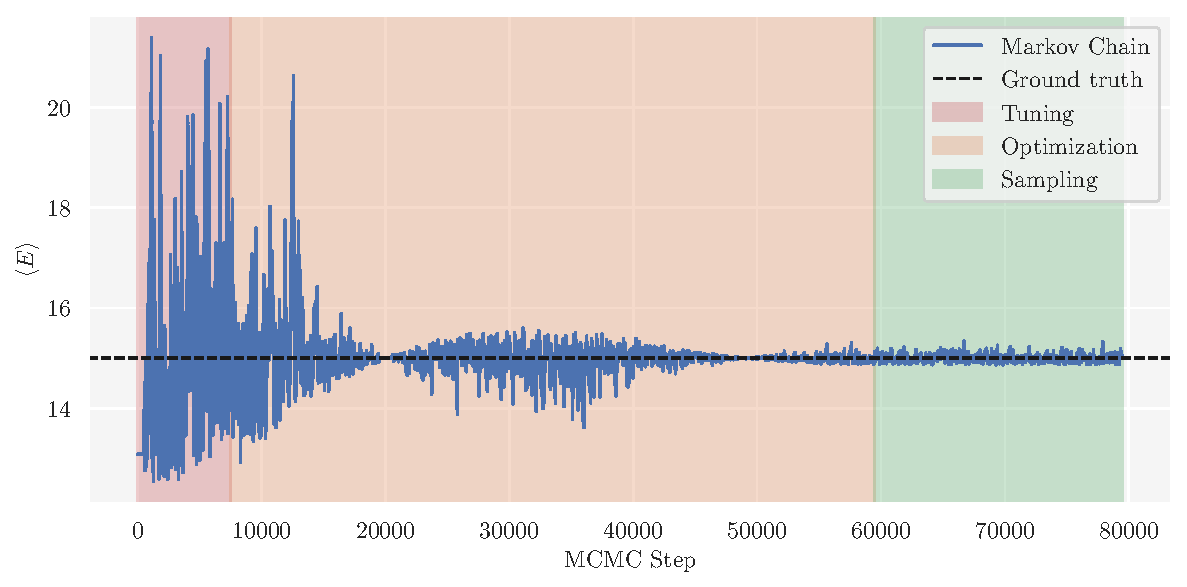
\includegraphics[scale=0.5]{latex/figures/trace_phase_rwm_ashonib.pdf}}}
\qquad
\subfloat[]{{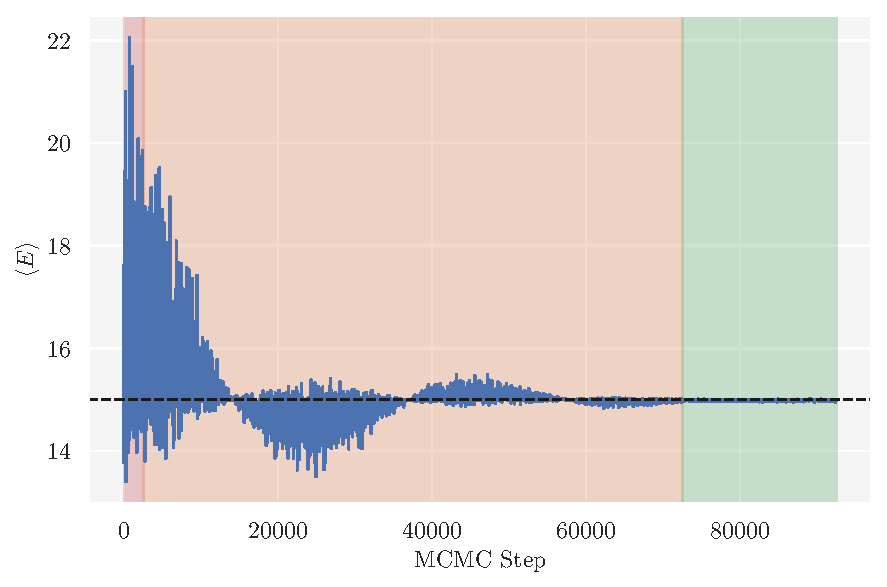
\includegraphics[scale=0.5]{latex/figures/trace_phase_lmh_ashonib.pdf}}}
\qquad
\subfloat[]{{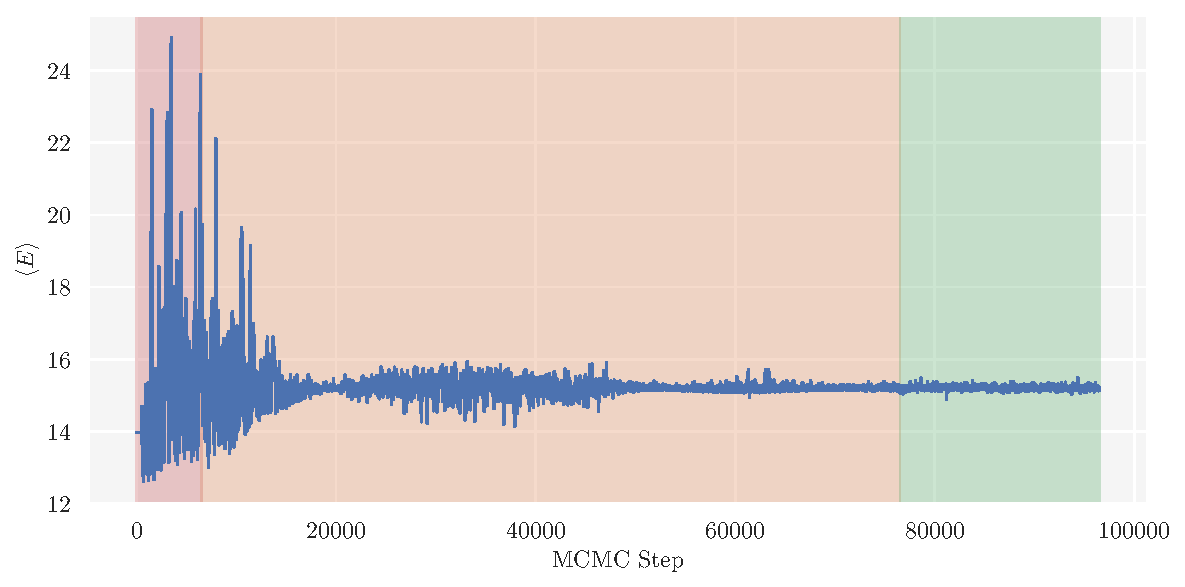
\includegraphics[scale=0.5]{latex/figures/trace_phase_rwm_ashoib.pdf}}}
\qquad
\subfloat[]{{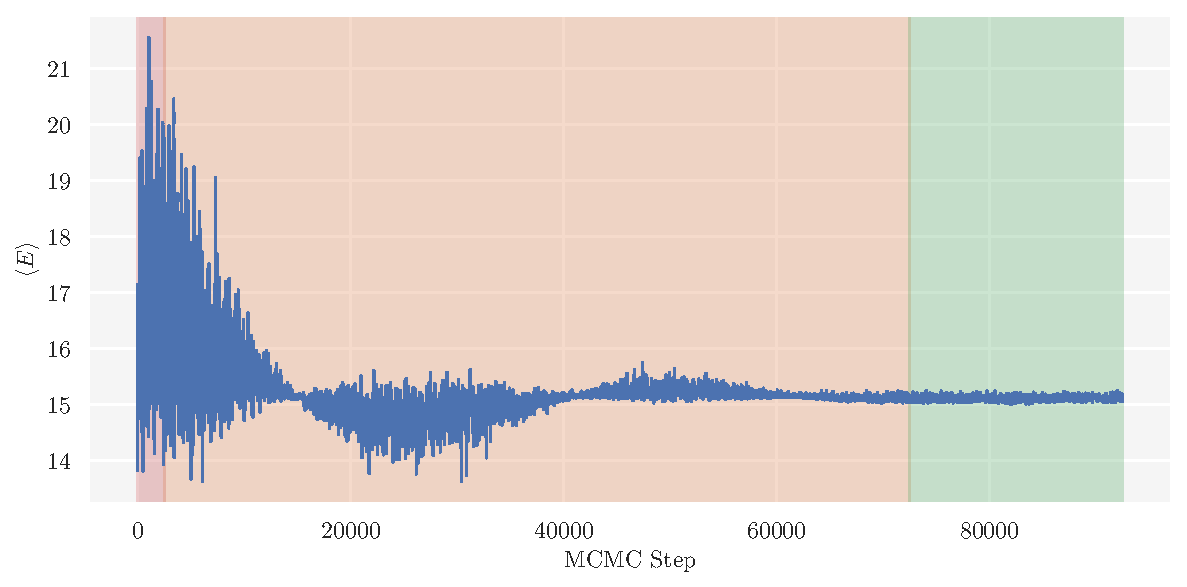
\includegraphics[scale=0.5]{latex/figures/trace_phase_lmh_ashoib.pdf}}}
\caption{The time evolution of a Markov chain in the three phases of the sampler; (i) tuning of the proposal scale parameter; (ii) gradient descent optimization of the variational parameter; and (iii) sampling of the variational energy. The updates in the tuning and optimization phase are done on a batch of samples, here 500 for tuning and 1000 for optimization. If the updated value remains the same between consecutive batches, the sampler will end the phase early. Here, the system consists of $N=100$ bosons in a spherical harmonic oscillator both with and without interactions. The initial variational parameter is set to $\alpha_0 = 0.4$. In \textbf{(a)} and \textbf{(b)} we see the RWM and LMH algorithm on a system of non-interacting bosons, respectively. In \textbf{(c)} and \textbf{(d)} we see the RWM and LMH algorithm on a system of interacting bosons, respectively.}
\label{fig:trace_phase}
\end{figure}




% Prevent floats going into the next (sub)section 
\FloatBarrier


%----------------------------------------------------------------
\subsection{Comparisons}
%----------------------------------------------------------------

\autoref{fig:alpha_epoch_rwm}

\begin{figure}[!htb]
\centering
\subfloat[]{{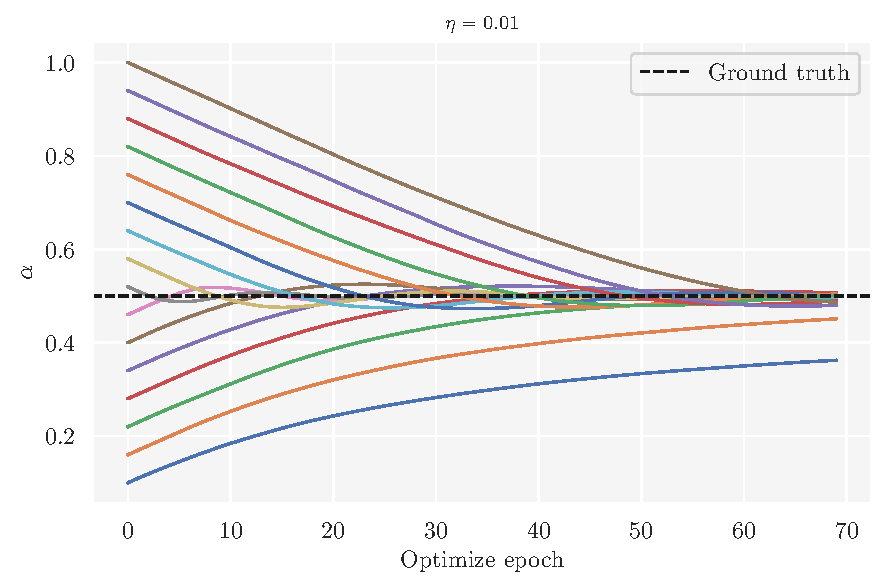
\includegraphics[scale=0.5]{latex/figures/alpha_epoch_rwm_ashonib_eta001.pdf}}}
\qquad
\subfloat[]{{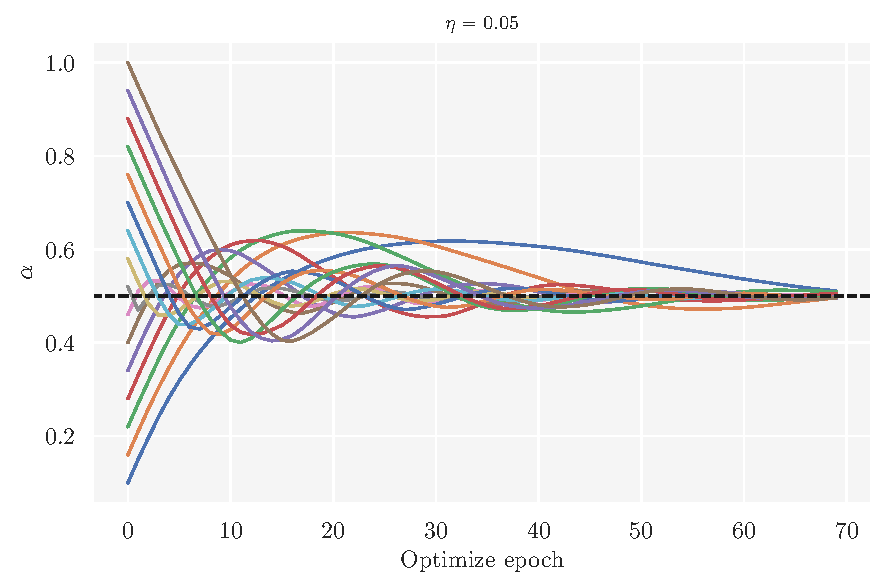
\includegraphics[scale=0.5]{latex/figures/alpha_epoch_rwm_ashonib_eta005.pdf}}}
\qquad
\subfloat[]{{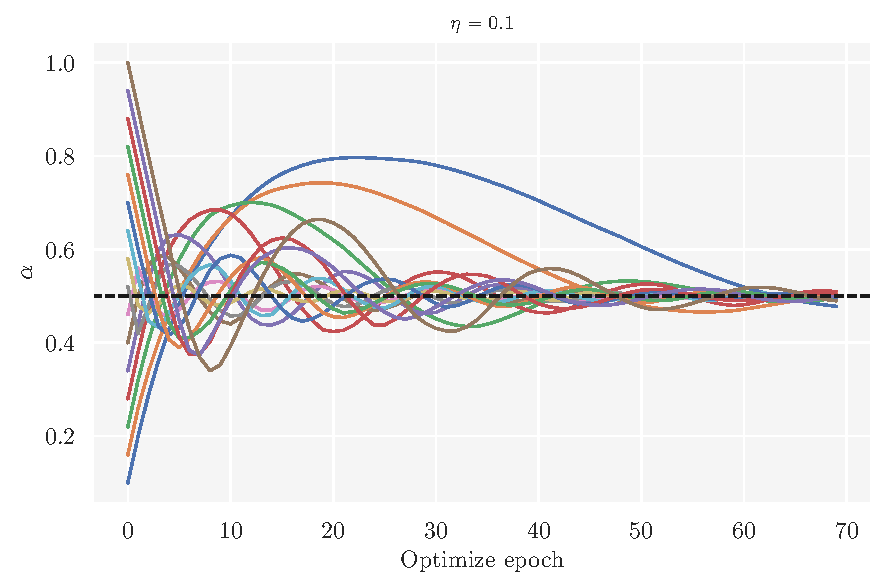
\includegraphics[scale=0.5]{latex/figures/alpha_epoch_rwm_ashonib_eta01.pdf}}}
\qquad
\subfloat[]{{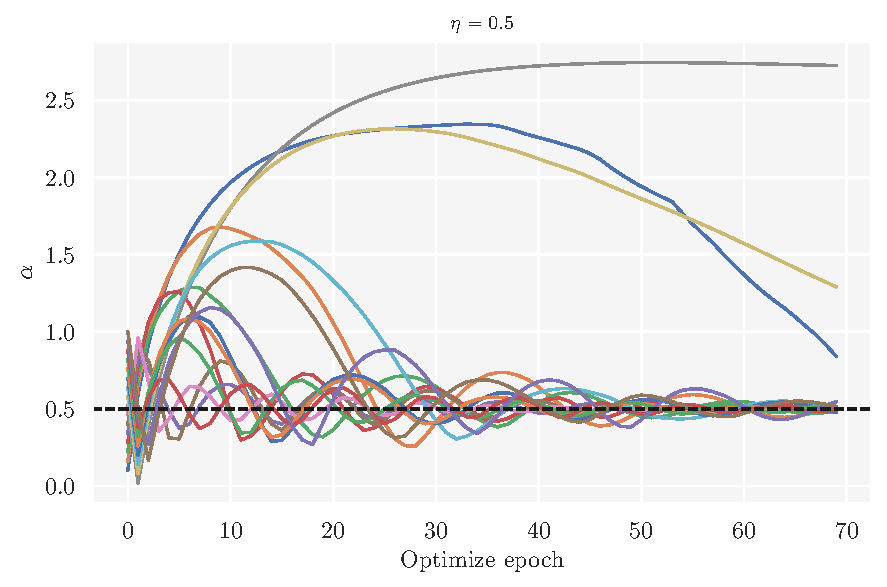
\includegraphics[scale=0.5]{latex/figures/alpha_epoch_rwm_ashonib_eta05.pdf}}}
\caption{figure text}
\label{fig:alpha_epoch_rwm}
\end{figure}

\autoref{fig:alpha_epoch_lmh}

\begin{figure}[!htb]
\centering
\subfloat[]{{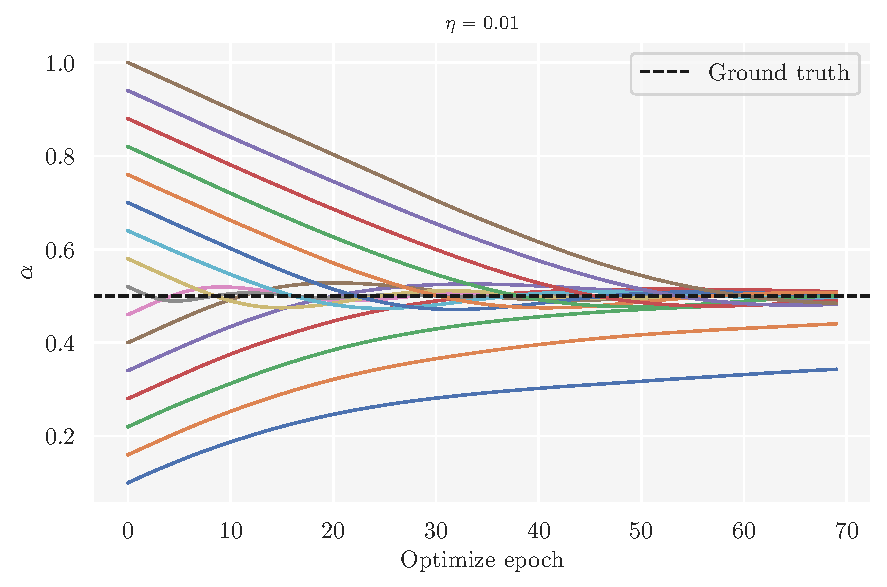
\includegraphics[scale=0.5]{latex/figures/alpha_epoch_lmh_ashonib_eta001.pdf}}}
\qquad
\subfloat[]{{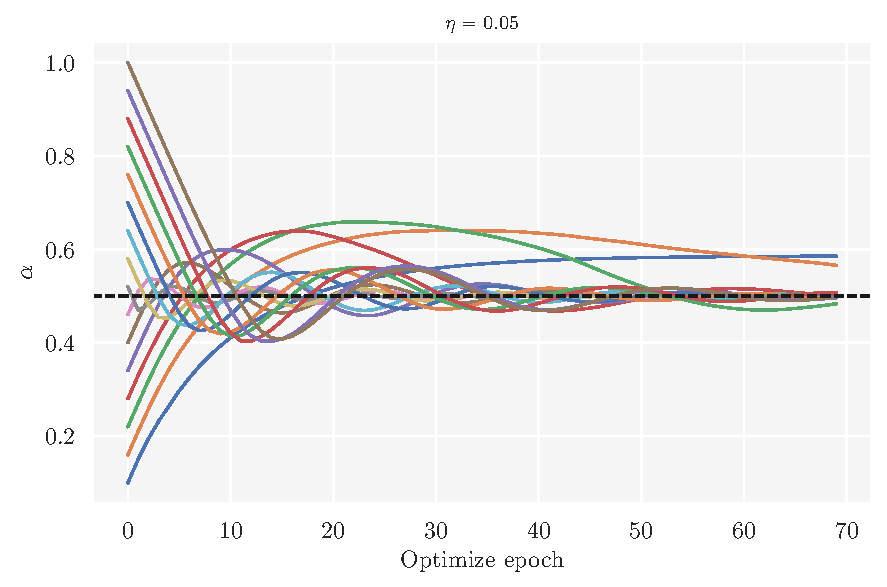
\includegraphics[scale=0.5]{latex/figures/alpha_epoch_lmh_ashonib_eta005.pdf}}}
\qquad
\subfloat[]{{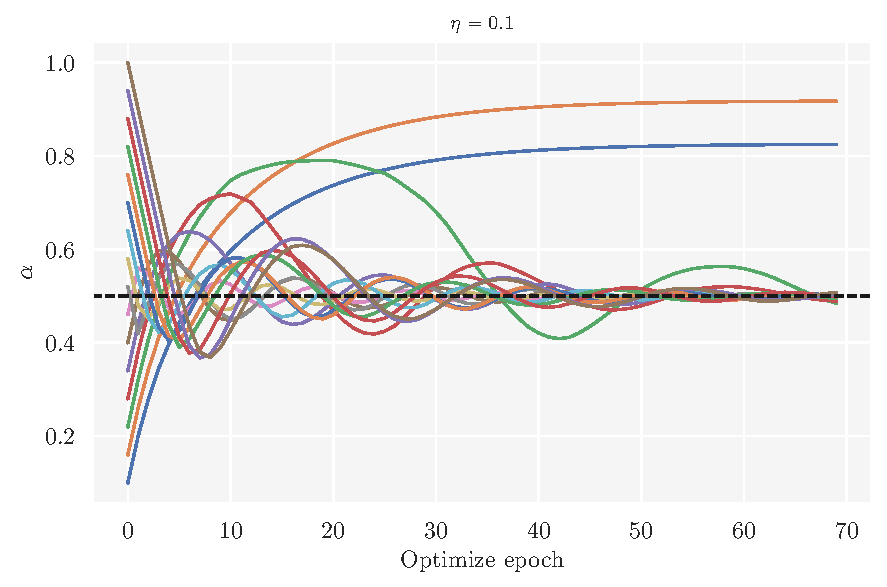
\includegraphics[scale=0.5]{latex/figures/alpha_epoch_lmh_ashonib_eta01.pdf}}}
\qquad
\subfloat[]{{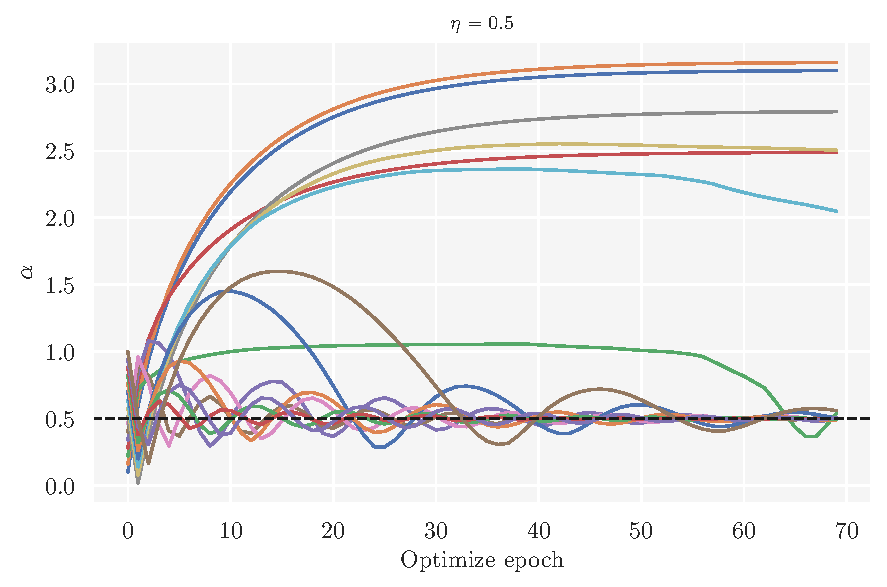
\includegraphics[scale=0.5]{latex/figures/alpha_epoch_lmh_ashonib_eta05.pdf}}}
\caption{figure text}
\label{fig:alpha_epoch_lmh}
\end{figure}

Comparing \autoref{fig:alpha_epoch_rwm} and \autoref{fig:alpha_epoch_lmh} - see no faster convergence of the variational parameter for LMH

 

Figure: Runtime RWM and LMH; Analytical vs JAX



%----------------------------------------------------------------
\subsection{Variational Energy}
%----------------------------------------------------------------

Figure : RWM and LMH Spherical non-interacting / interacting 

Figure: RWM LMH Elliptical non-interacting / interacting  

%----------------------------------------------------------------
\subsection{OBD}
%----------------------------------------------------------------


Move figures below here



%%
%%
%%

%----------------------------------------------------------------
\subsubsection{Non-Interacting}
%----------------------------------------------------------------

\textbf{Spherical potential}

Discussion

\autoref{fig:non-interact_boxplot} shows 

\begin{figure}[!htb]
\centering
\subfloat[]{{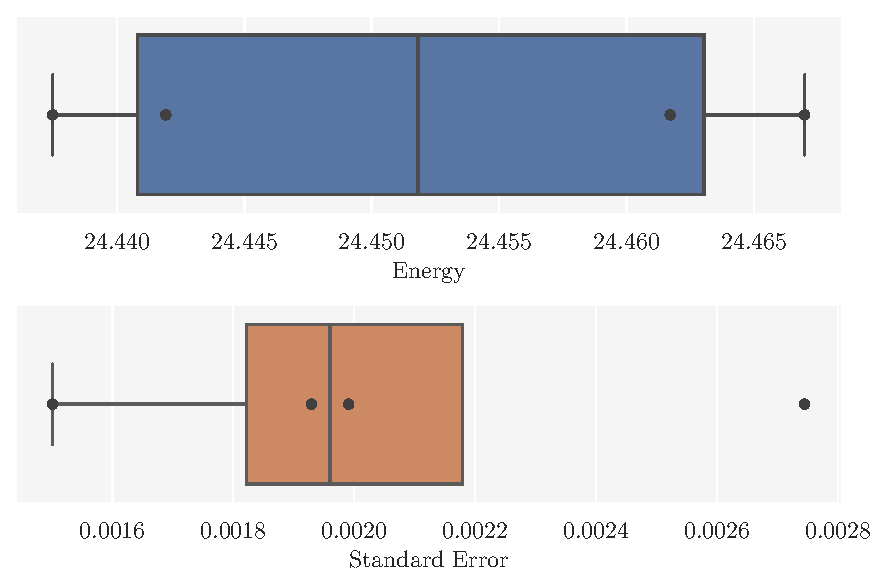
\includegraphics[scale=0.5]{latex/figures/boxplot_analytical_metropolis.pdf}}}
\qquad
\subfloat[]{{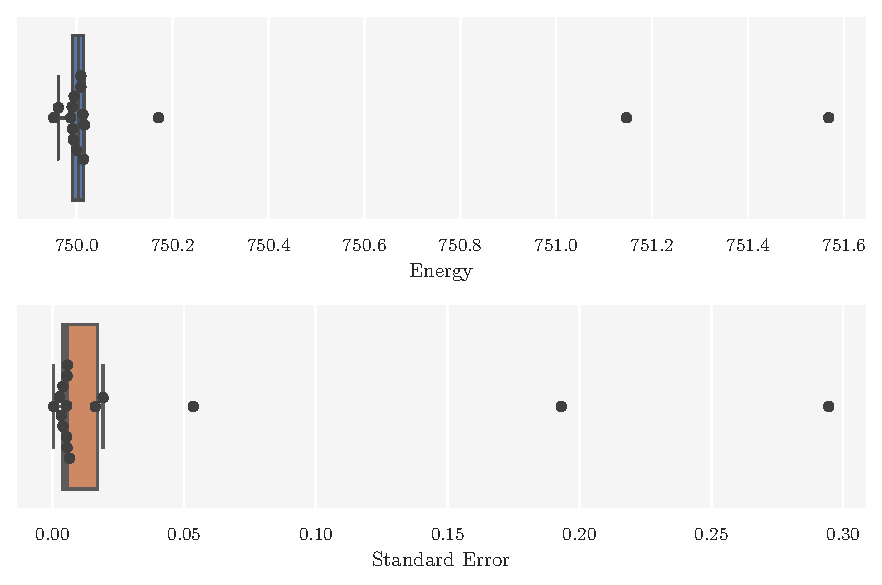
\includegraphics[scale=0.5]{latex/figures/boxplot_analytical_metropolis_hastings.pdf}}}
\qquad
\subfloat[]{{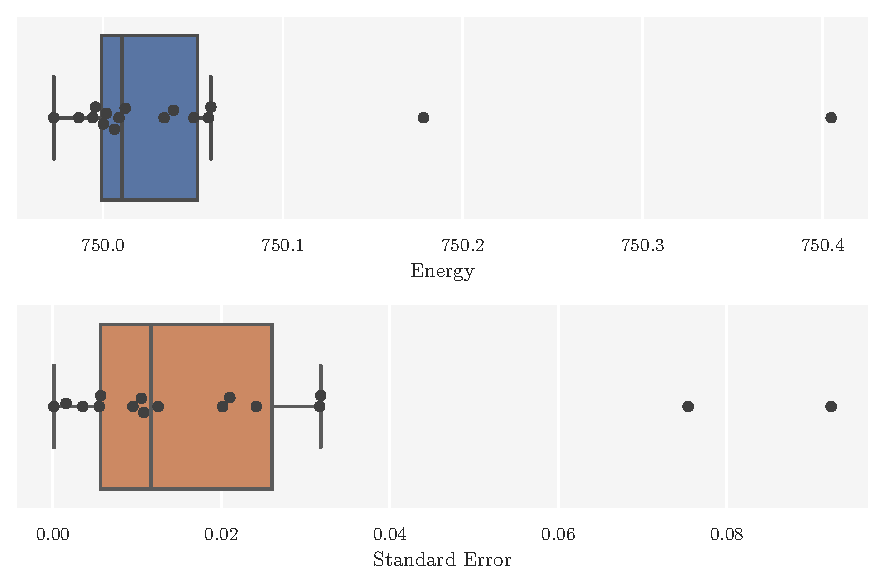
\includegraphics[scale=0.5]{latex/figures/boxplot_numerical_metropolis.pdf}}}
\qquad
\subfloat[]{{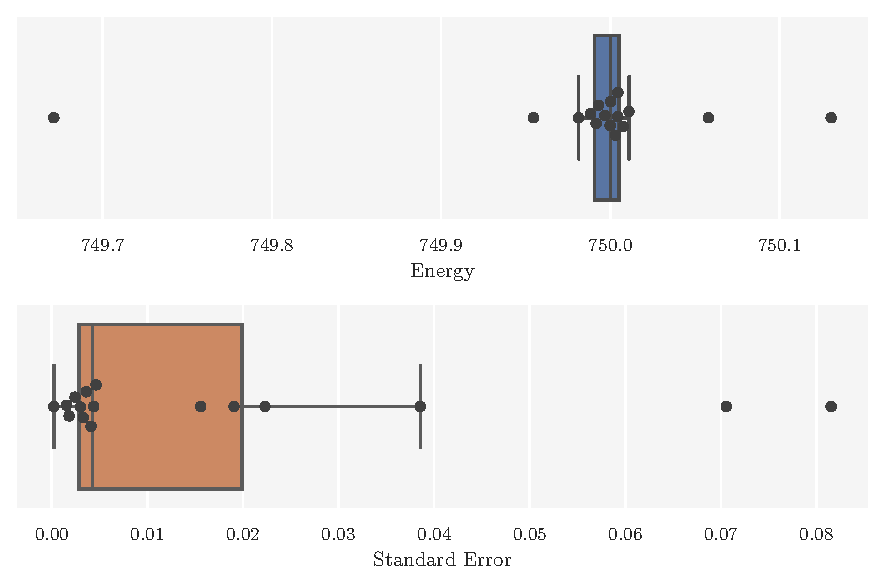
\includegraphics[scale=0.5]{latex/figures/boxplot_numerical_metropolis_hastings.pdf}}}
\caption{\textbf{(a)} Random Walk Metropolis with analytical. \textbf{(b)} Langevin Metropolis-Hastings with analytical. \textbf{(c)} Random Walk Metropolis with AD. \textbf{(d)} Langevin Metropolis-Hastings with AD.}
\label{fig:non-interact_boxplot}
\end{figure}

\textbf{Elliptical potential}
The ground state energy of the non-interacting particles in the elliptical potential with $\beta=2.82843$ is $\frac{\expval{E}}{N}=2.414215\hbar\omega_0$, and the ground state $\alpha=0.5$, as in the spherical potential. 



%----------------------------------------------------------------
\subsubsection{Interacting}
%----------------------------------------------------------------

\textbf{Spherical potential}

In \autoref{fig:interactions_plot} variational grid searches for the non-interacting case, and $10, 50, 100$ particles with interactions are shown. The $y$-axis displays the energy per particle. A $95$\% confidence interval is shaded in light blue. The minimal energy per particle values together with their standard error, $\sigma$, are tabulated in \autoref{tab:min_energies}. 
\begin{figure}[!htb]
\centering
\subfloat[]{{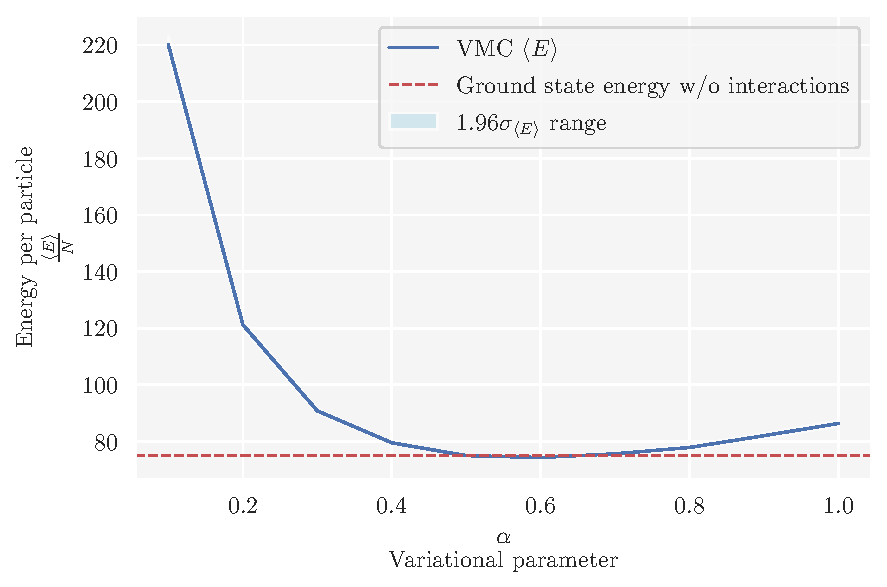
\includegraphics[scale=0.5]{latex/figures/grid_search_analytical_wo_interactions_N_50.pdf}}}
\qquad
\subfloat[]{{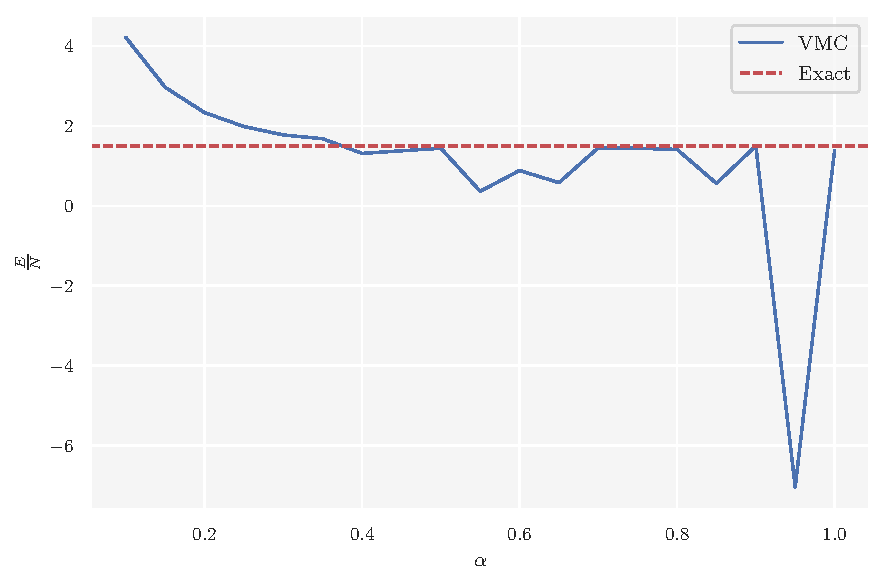
\includegraphics[scale=0.5]{latex/figures/grid_search_analytical_w_interactions_N_10.pdf}}}
\qquad
\subfloat[]{{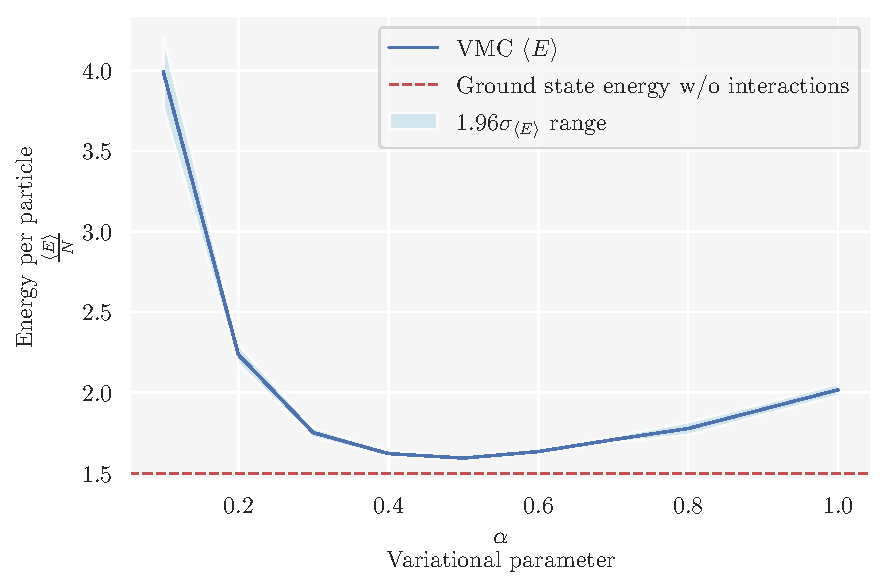
\includegraphics[scale=0.5]{latex/figures/grid_search_analytical_w_interactions_N_50.pdf}}}
\qquad
\subfloat[]{{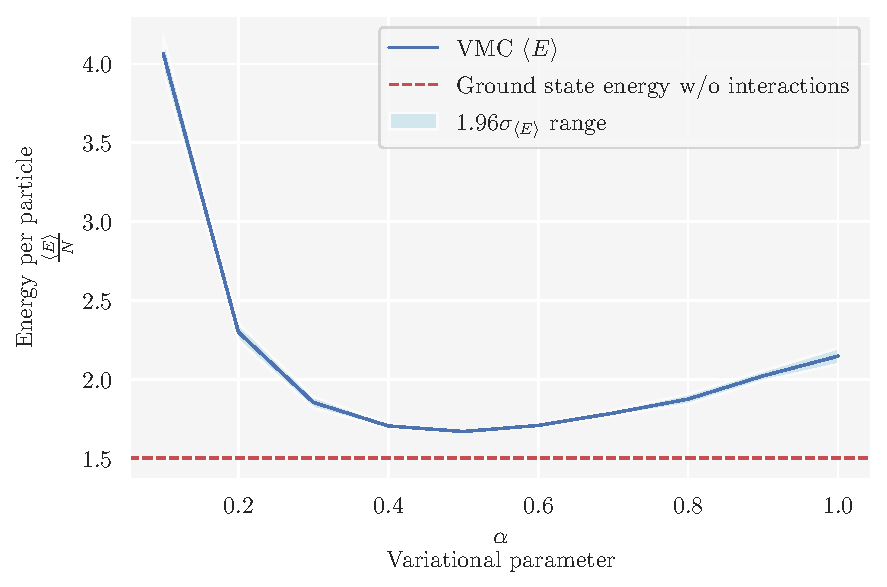
\includegraphics[scale=0.5]{latex/figures/grid_search_analytical_w_interactions_N_100.pdf}}}
\caption{\textbf{(a)} Random Walk Metropolis with 50 non-interacting particles. \textbf{(b)} Random Walk Metropolis with ten interacting particles. \textbf{(c)} Random Walk Metropolis with 50 interacting particles. \textbf{(d)} Random Walk Metropolis with 100 interacting particles.}
\label{fig:interactions_plot}
\end{figure}

\begin{table}[H]
    \centering
    \begin{tabular}{ccccc}
    \hline \hline
        Number of particles & Interactions & $\frac{\expval{E}_{\mathrm{min}}}{N}$ & $\sigma$ & $\alpha^{\mathrm{opt}}$\\
    \hline \hline
        $50$ & Off & $1.500$ & $0\cdot10^{0}$ & $0.5$\\
        $10$ & On & $1.51731$& $8\cdot10^{-5}$& $0.5$ \\
        $50$ & On & $1.59490$& $3\cdot10^{-4}$ &$0.5$ \\
        $100$ & On & $1.66912$ & $3\cdot10^{-4}$ & $0.5$ \\
    \hline \hline
    \end{tabular}
    \caption{The minimal energies of the grid searches for $10, 50, 100$ particles, together with the standard error and the optimal $\alpha$ values. The interactions column displays whether or not the particles are interacting with one another.}
    \label{tab:min_energies}
\end{table}

As you can see in \autoref{tab:min_energies}, the minimal energy per particle is increasing with the number of particles when they are interacting. The density of particles within the potential increases with the number of particles unleashed in the same potential. This leads to more interactions between the particles, and thus a higher energy. Another important quantity, the standard error, is represented with the $95$\% confidence interval $[\mu\pm1.96\sigma]$ by the shaded light blue in \autoref{fig:interactions_plot}. The standard error is relatively small, but it should be possible to see the convex nature of it. It is decreasing from $\alpha=0.1\to\alpha=0.5$, where it increases again. 


\autoref{fig:comparisons_interactions_plot} displays the VMC calculations of the grid searches in \autoref{fig:interactions_plot} all together in one plot. This way it is easier to see the increase in energy per particle as a function of the number of interacting particles. 

\begin{figure}[H]
\begin{center}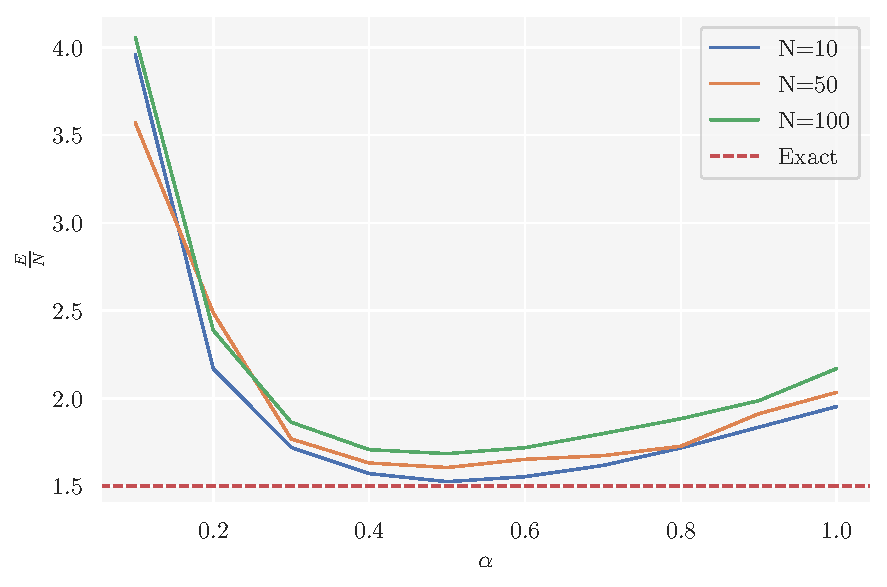
\includegraphics[scale=1.0]{latex/figures/grid_search_analytical_w_interactions_all_N.pdf}
\end{center}
\caption{Random Walk Metropolis energy per particle comparison between $N=10, 50, 100$ interacting particles, and $N=50$ non-interacting particles.}
\label{fig:comparisons_interactions_plot}
\end{figure}

\subsubsection{One-body densities}
\autoref{fig:one_body_densities} shows the sampled one body densities for $10$ and $100$ particles with interactions turned on and off. As the number of particles increases, the density of particles increases, and the interactions between the particles becomes a larger factor. For $10$ particles, the one body densities with and without interactions are almost identical. This means that for $10$ particles, the interactions do not have a large impact on the system. For $100$ particles, the radial one body densities for the interacting and non-interacting cases differ more. The particles in the interacting case are more spread out in the $2$-dimensional space than the non-interacting case. The interactions makes quite a difference when there are $100$ particles. 
\begin{figure}[H]
\centering
\subfloat[]{{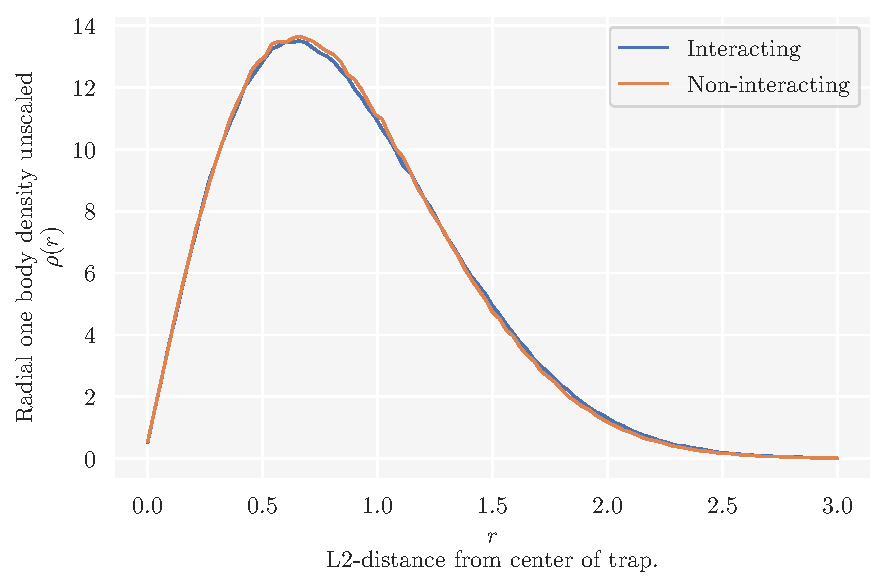
\includegraphics[scale=0.5]{latex/figures/OBD_N10.pdf}}} 
\qquad
\subfloat[]{{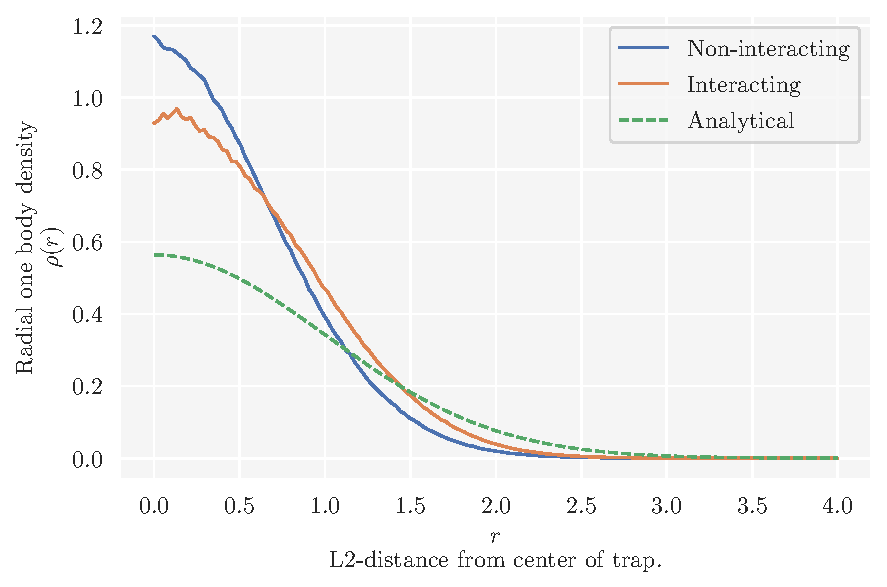
\includegraphics[scale=0.5]{latex/figures/OBD_N100.pdf}}}
\caption{\textbf{(a)} Comparison between the radial one body densities for $10$ particles with and without interactions (Jastrow factor $a=0.00433$) in $2$-dimensional space. \textbf{(b)} Comparison between the radial one body densities for $100$ particles with and without interactions (Jastrow factor $a=0.00433$) in $2$-dimensional space.}
\label{fig:one_body_densities}
\end{figure}

\textbf{Elliptical potential}

\autoref{fig:energy_elliptical} displays 16 independent energy sampling runs where $\alpha$ is optimized. 

\begin{figure}[H]
\begin{center}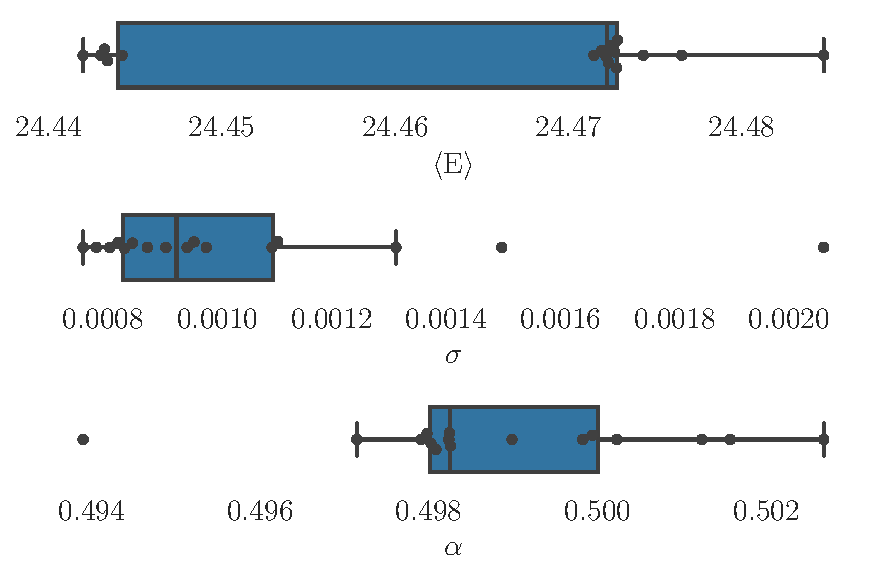
\includegraphics[scale=0.5]{figures/aehoib_bp.pdf}
\end{center}
\caption{Sampled energies, the standard errors and the optimized $\alpha$-values of $16$ independent sampling runs.}
\label{fig:bp_aehoib}
\end{figure}

RWM vs LMH - standard error

In \autoref{fig:comparison_se_RWMvLMH} the evolution of the standard error is plotted as a function of the logarithm with base $2$ of the number of samples, $\log_2{M}$. The numbers of samples used is from $2^{10}\to2^{20}$ where the number of samples increases by a factor of two in each step. \autoref{fig:comparison_time_RWMvLMH} displays the time spent sampling for each run. We have used the same number of warm-up cycles. The number of tuning cycles may differ, but it is of a relatively small order compared with warm-ups and sampling. 

\begin{figure}[H]
\begin{center}\includegraphics[scale=0.5]{Figures/filename}
\end{center}
\caption{The standard error as a functions of the base $2$ logarithm of the number of energy samples. The blue line represents the Random Walk Metropolis sampling algorithm, while the orange represents the Langevin Metropolis-Hastings sampling algorithm.}
\label{fig:comparison_se_RWMvLMH}
\end{figure}

\begin{figure}[H]
\begin{center}\includegraphics[scale=0.5]{Figures/filename}
\end{center}
\caption{Time spent running the sampling algorithm as a functions of the base $2$ logarithm of the number of energy samples. The blue line represents the Random Walk Metropolis sampling algorithm, while the orange represents the Langevin Metropolis-Hastings sampling algorithm.}
\label{fig:comparison_time_RWMvLMH}
\end{figure}
